\documentclass[a4paper]{article}
\usepackage[italian]{babel}

% immagini
\usepackage{graphicx}
\usepackage{svg}
\usepackage{amsthm}

% matematica
\usepackage{amsmath}
\usepackage{amsfonts}

% codice
\usepackage{listings}
\lstset{
    basicstyle=\small\ttfamily,
    numbers=left,
    numberstyle=\small\ttfamily
}

% \usepackage{blindtext}
\usepackage{titlesec}
% \usepackage{geometry}
% \usepackage{relsize}
\usepackage{tikz}
% \geometry{
% a4paper,
% total={190mm,257mm},
% left=25mm,
% right=25mm,
% top=50mm,
% }

\usepackage{hyperref}

% \sloppy % ?

% comandi per riferirsi agli algoritmi
\newcommand{\QuickSelect}{\textsc{QuickSelect}}
\newcommand{\HeapSelect}{\textsc{HeapSelect}}
\newcommand{\MoMSelect}{\textsc{MoMSelect}}

% comandi per la notazione asintotica
\newcommand{\Tquad}{\ifmmode \Theta(n^2) \else $\Theta(n^2)$\fi} % Θ(n^2)
\newcommand{\Tlin}{\ifmmode \Theta(n) \else $\Theta(n)$\fi} % Θ(n)
\newcommand{\Olin}{\ifmmode O(n) \else $O(n)$\fi} % O(n)

\begin{document}

\begin{titlepage} % pagina riservata al titolo
    \begin{center}
        \vspace*{1cm}
        {\Huge\bfseries Analisi di algoritmi di selezione\par}
        \vspace{.5cm}
        {\LARGE Progetto di laboratorio di Algoritmi e Strutture Dati\par}
        \vspace{1cm}
        \begin{figure}[h]
            \centering
            
\includegraphics[width=.5\textwidth]{photo/uniud_logo.png}
        \end{figure}
        \vspace{1.5cm}
        {\LARGE Università degli studi di Udine\par}
        {\LARGE Dipartimento di scienze Informatiche, Matematiche e Fisiche\par}
        \vfill
        {\Large Anno Accademico 2023/2024\par}
        {\Large Matricole: 162367, 162473, 162013\par}
        {\Large\itshape Gerardi Ludovico, Sclauzero Lorenzo, Pantanali Riccardo\par}
    \end{center}
\end{titlepage}



\section{Introduzione}
Il progetto ha come scopo l'implementazione di tre algoritmi di selezione e l'analisi della loro complessità. 
Dato un vettore di interi $v$ di dimensione $n$ e un intero $k$ con $1 < k \le n$, gli algoritmi di selezione calcolano il $k$-esimo elemento più piccolo di $v$.

I tre algoritmi discussi sono \QuickSelect{}, \HeapSelect{} e \MoMSelect{} (che sta per median-of-medians select); vengono presentati nella sezione \ref{sec:presentazione-algoritmi} insieme all'algoritmo utilizzato per la generazione dell'input.
Nella sezione \ref{sec:misurazione} si discute brevemente la misurazione dei tempi di esecuzione, necessaria per l'analisi della complessità.
Nella sezione \ref{sec:grafici} vengono presentati e discussi i risultati delle misurazioni sotto forma di grafici.
Infine nella sezione \ref{sec:confronto-mom} viene proposto un confronto tra alcune varianti di \MoMSelect{}.



\section{Presentazione degli algoritmi}
\label{sec:presentazione-algoritmi}

\subsection{Algoritmi di selezione}
\paragraph{\QuickSelect}
Questo algoritmo partiziona ricorsivamente $v$ rispetto a un elemento scelto come pivot e confronta la posizione finale del pivot con $k$: sono sono uguali allora l'algoritmo termina, ritornando $v[k]$; altrimenti effettua una chiamata ricorsiva sulla partizione sinistra o destra di $v$, a seconda che $k$ sia rispettivamente minore o maggiore della posizione finale del pivot.
Quest'ultimo viene scelto sempre come l'ultimo elemento del sottovettore considerato.
Tale approccio porta la complessità nel caso peggiore a essere \Tquad{} (quando il vettore è già ordinato, in un senso o nell'altro), mentre nel caso medio è \Tlin.
D'altra parte l'overhead dovuto alla scelta del pivot è molto basso, il che, come si vedrà, porta ad un vantaggio rispetto a \MoMSelect{} nel caso di vettore generati pseudocasualmente.

\paragraph{\HeapSelect}
\HeapSelect{} utilizza due heap $H_1$ e $H_2$.
$H_1$ è una min-heap che viene costruita a partire da $v$ in tempo lineare e non viene successivamente modificata.
$H_2$ è una min-heap che inizialmente contiene solo il nodo radice di $H_1$.
Ad ogni iterazione viene estratta la radice $r$ da $H_2$ e vengono aggiunti i figli di $r$ in $H_1$ all'interno di $H_2$.
Dopo $k-1$ iterazioni $r$ è l'elemento cercato, cioè il $k$-esimo più piccolo all'interno di $v$.
Siccome cercare il $k$-esimo elemento più piccolo equivale a cercare l'elemento $(n-k+1)$-esimo più grande, se $k>n/2$ è si utilizza una max-heap per $H_2$, il che consente di ridurre il numero di iterazioni necessarie.
Questo algoritmo ha una complessità temporale pari a $O(n+k\log k)$ sia nel caso pessimo che in quello medio.

\paragraph{\MoMSelect}
Il funzionamento ad alto livello di \MoMSelect è come quello di \QuickSelect: effettuare una chiamata ricorsiva sulla porzione di vettore che contiene l'elemento cercato.
La differenza tra i due algoritmo sta nella scelta del pivot.
Infatti \MoMSelect{} utilizza una procedura ausiliaria che calcola la posizione della mediana delle mediana all'interno del sottovettore considerato.
Nello specifico tale procedura divide il vettore in blocchi da $5$ elementi (eccetto al più l'ultimo blocco), ordina ciasun blocco e ne calcola la mediana, e quindi effettua una chiamata ricorsiva sulle mediane appena calcolate finché non rimane un solo elemento: la mediana delle mediane.
Sono proposte tre varianti:
\begin{enumerate}
    \item non in-place: alloca un nuovo vettore ad ogni chiamata ricorsiva per memorizzare le mediane dei blocchi;
    \item quasi in-place: riutilizza lo spazio allocato per il vettore originariamente fornito in input;
    \item in-place: riutilizza lo spazio del vettore originario, come nella variante precedente, ma senza effettuare chiamate ricorsive.
\end{enumerate}

In tutti i casi, la complessità temporale e spaziale dell'algoritmo nel caso pessimo è \Olin. 
Nei grafici della sezione \ref{sec:grafici} verrà utilizzata la versione quasi in Place.

\subsection{Algoritmo per la generazione dei vettori}
La lunghezza $n$ del vettori generati varia da $1000$ ($n_{\min}$) a $100000$ ($n_{\max}$), mentre i valori degli interi variano $0$ a $100000$.
In certe misurazioni la lunghezza dei vettori cresce secondo la serie geometrica
\[
    L(i) = n_{\min} \cdot \left(\frac{n_{\max}}{n_{\min}}\right)^{i/99}
\]
dove $i$ è il numero dell'iterazione corrente, che varia da $0$ a $99$, per un totale di $100$ iterazioni.
Si noti in particolare che $L(0) = n_{\min}$ e $L(99) = n_{\max}$.


\section{Misurazione dei tempi di esecuzione}
\label{sec:misurazione}
La misurazione dei tempi necessari per calcolare il k-esimo numero in un array viene effettuata considerando la lunghezza \( n \) dell'array di input e l'errore massimo consentito. Per ogni lunghezza dell'array, gli algoritmi implementati ripetono il calcolo del k-esimo numero un numero di volte tale da garantire un errore massimo relativo pari a \( f_{\max} = 0.001 \), assicurando così un tempo totale maggiore o uguale a \( T_{\min} \), calcolato come \[ T_{\min} = R \left( \frac{1}{f} + 1 \right) \] dove \( R \) rappresenta la risoluzione del clock.

Ciascuna iterazione del calcolo del k-esimo numero viene eseguita su un array generato pseudo-casualmente di lunghezza \( n \), differente ad ogni iterazione.
L'analisi dell'efficienza dei tre algoritmi viene effettuata attraverso la misurazione dei tempi medi\\

\newpage
\section{Rappresentazione grafica dei risultati}
\label{sec:grafici}

\subsection{Caso k costante}
\begin{figure}[h]
            \centering
            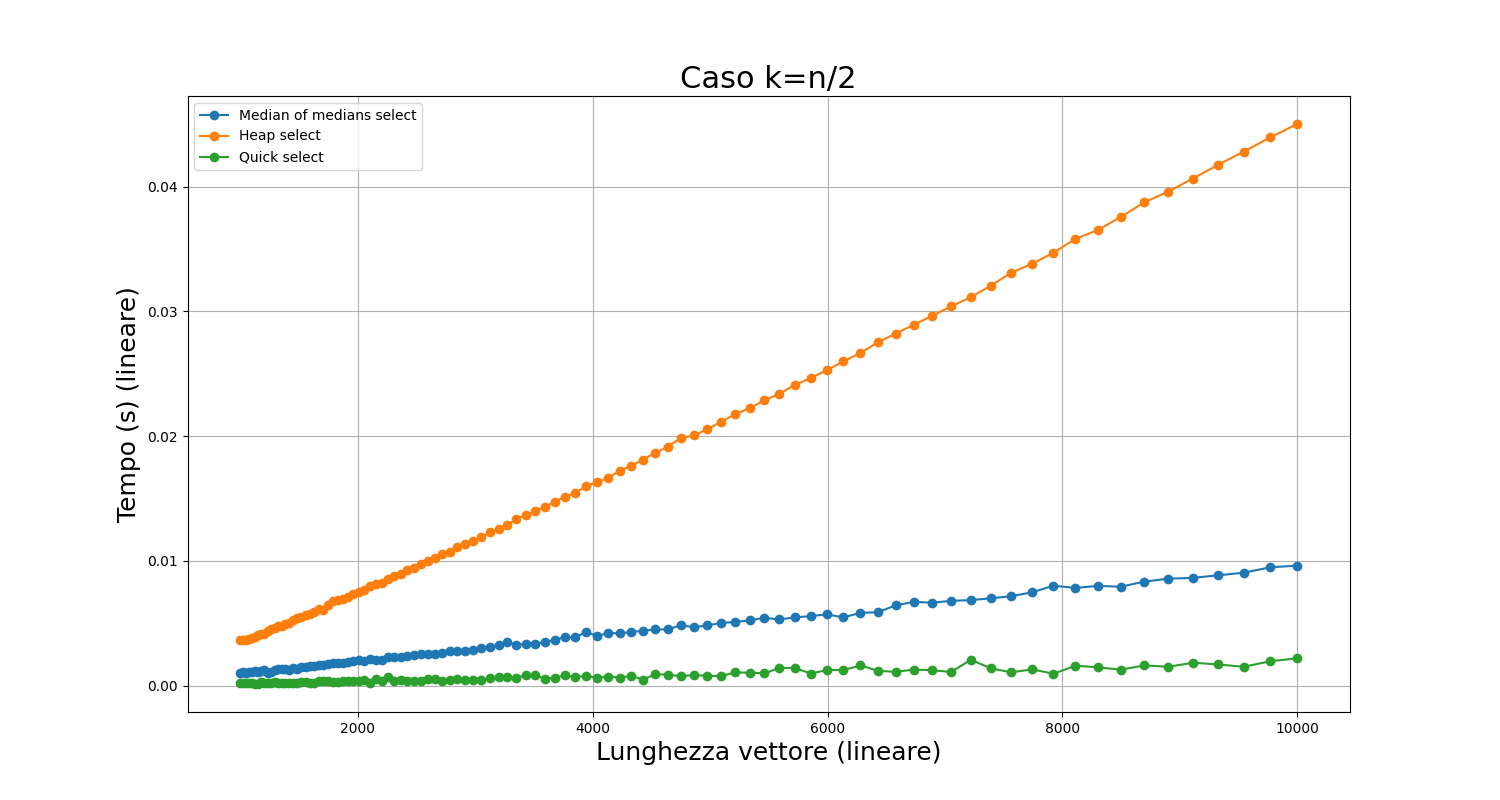
\includegraphics[width=.83\textwidth]{graphs/k_const_n.png}
            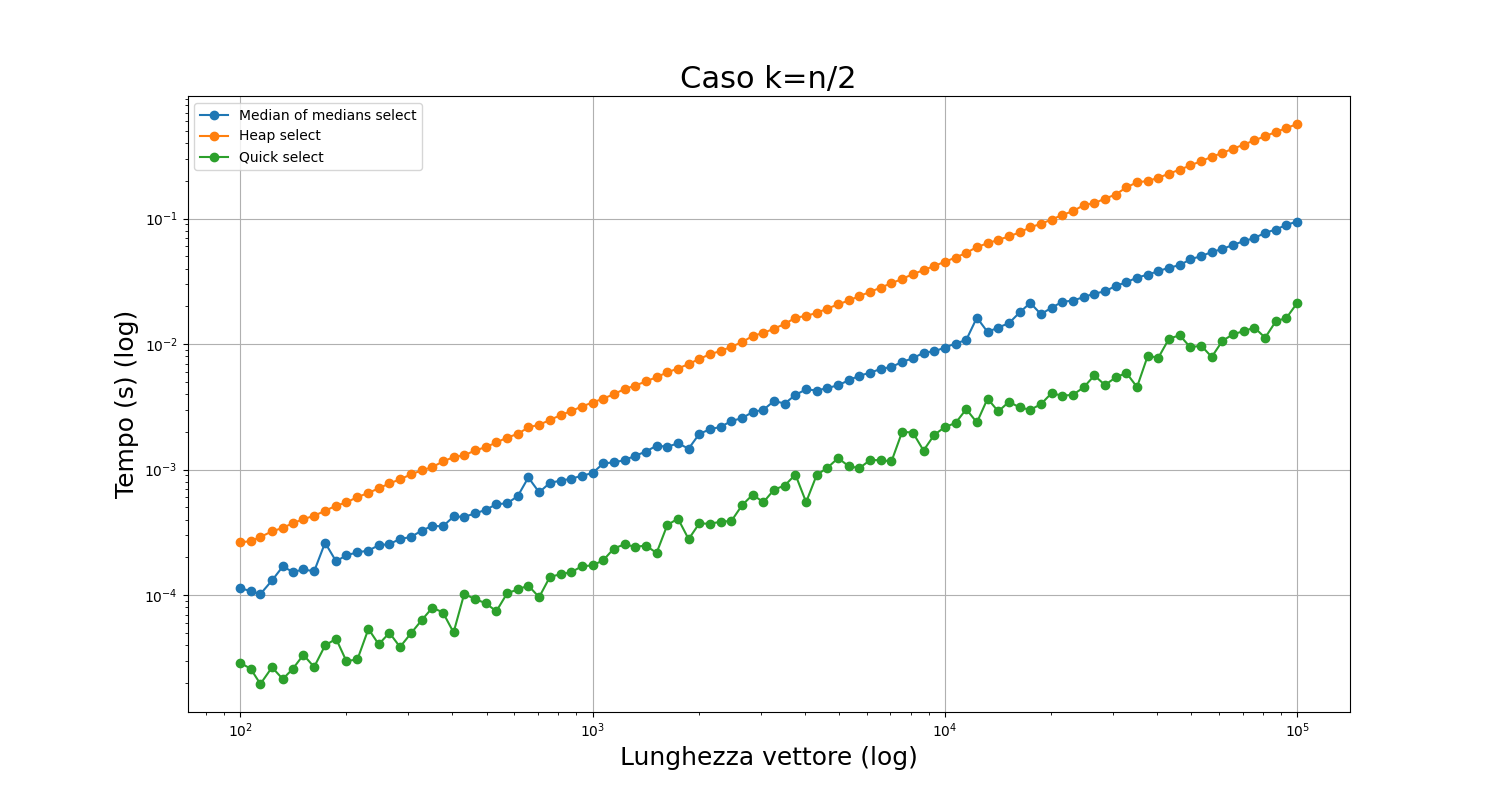
\includegraphics[width=.83\textwidth]{graphs/k_const_2xlog.png}
\end{figure}
Come si può notare dai grafici, con $k=\frac{n}{2}$ l'algoritmo $HeapSelect$ risulta essere quello con prestazioni peggiori tra i tre assumendo un andamento dell'oridine di $klogk$.
$Medians\ Of\ Medians$ e $Quick\ Select$ hanno entrambi complessita $O(n)$ però $MoM$ ha un andamento peggiore a causa degli ulteriori calcoli per determinare la mediana delle mediane.\\
\newpage
\begin{figure}[h]
            \centering
            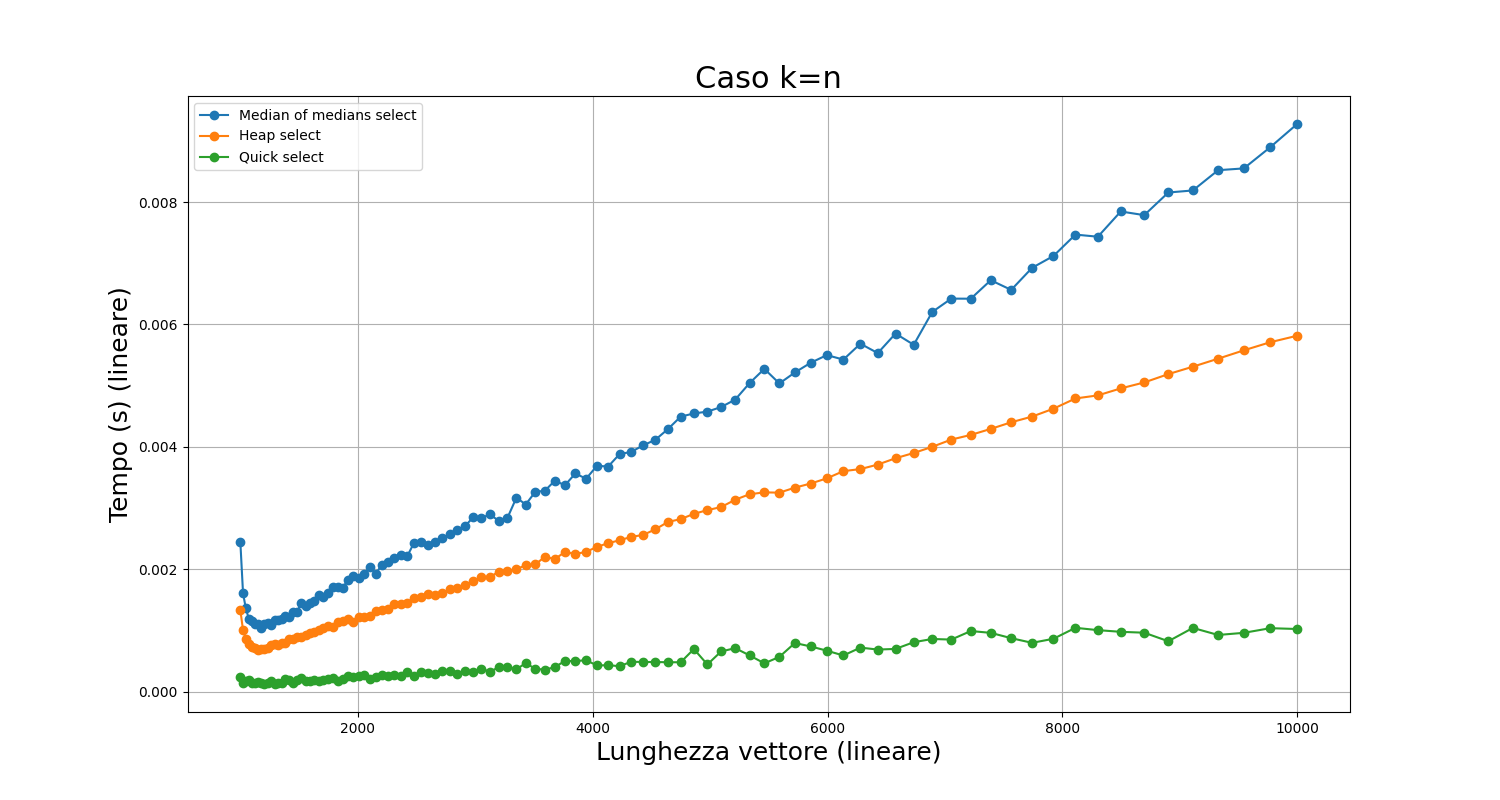
\includegraphics[width=.83\textwidth]{graphs/k_last_n.png}
            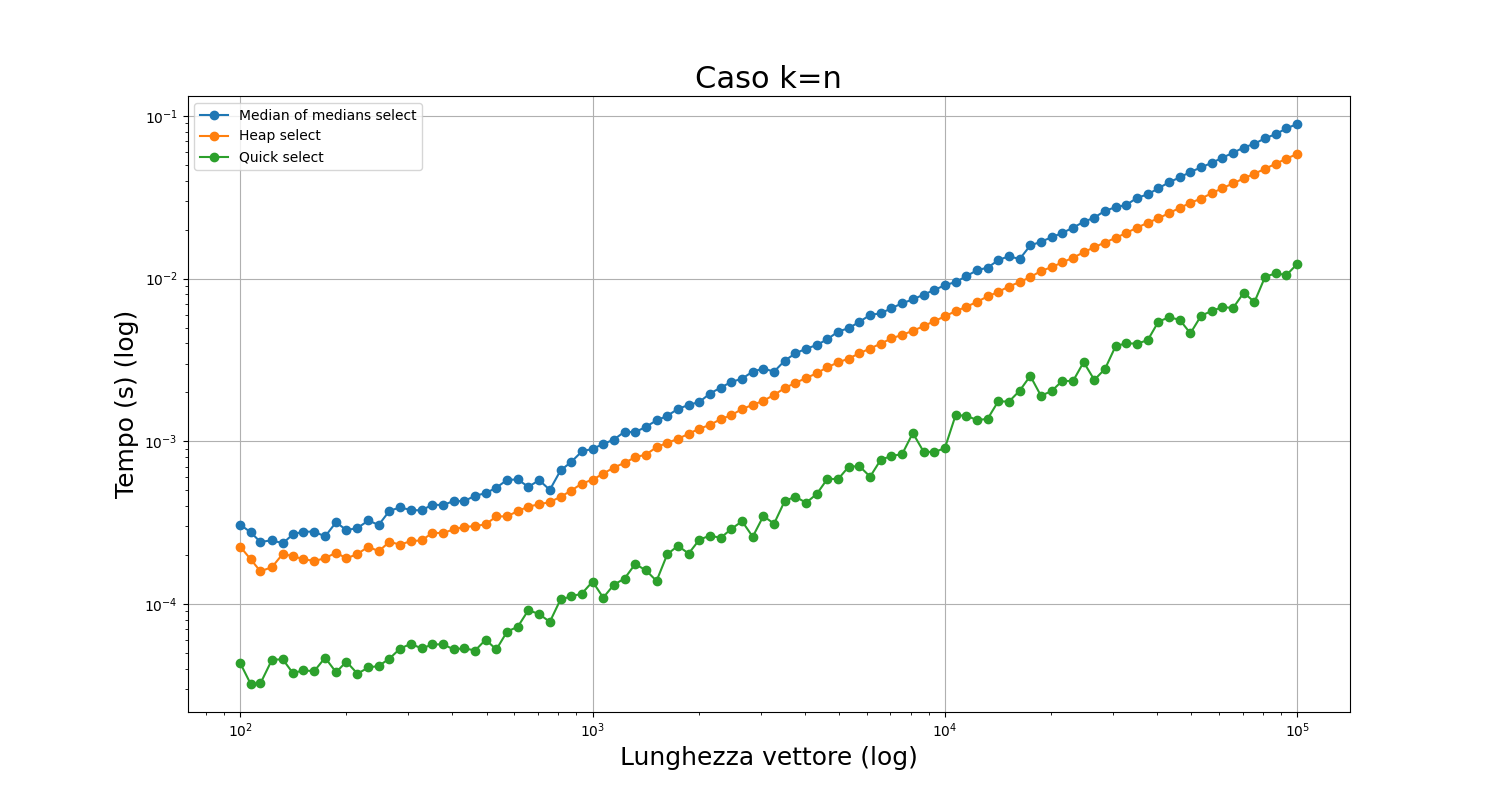
\includegraphics[width=.83\textwidth]{graphs/k_last_2xlog.png}
\end{figure}
Come si evince dal grafico nel caso in cui $k$ risulti posizionarisi a uno dei due estremi del vettore porta a un netto miglioramento delle perfomance da parte di $Heap\ Select$.\\
Questo è dovuto dal fatto come spiegato nella sezione 2.1 che a seconda della posizione di k se $k\in[0,\frac{n}{2}]$ viene adottata una MinHeap mentre se $k\in[\frac{n}{2}+1,n-1]$ viene utilizzata un MaxHeap, adottando un andamento lineare nel caso in cui k tenda agli estremi del vettore.\\
Mentre gli andamenti di $MoM$ e $Quick\ Select$ rimangono invarianti.\\
\newpage
\subsection{Caso k random}
\begin{figure}[h]
            \centering
            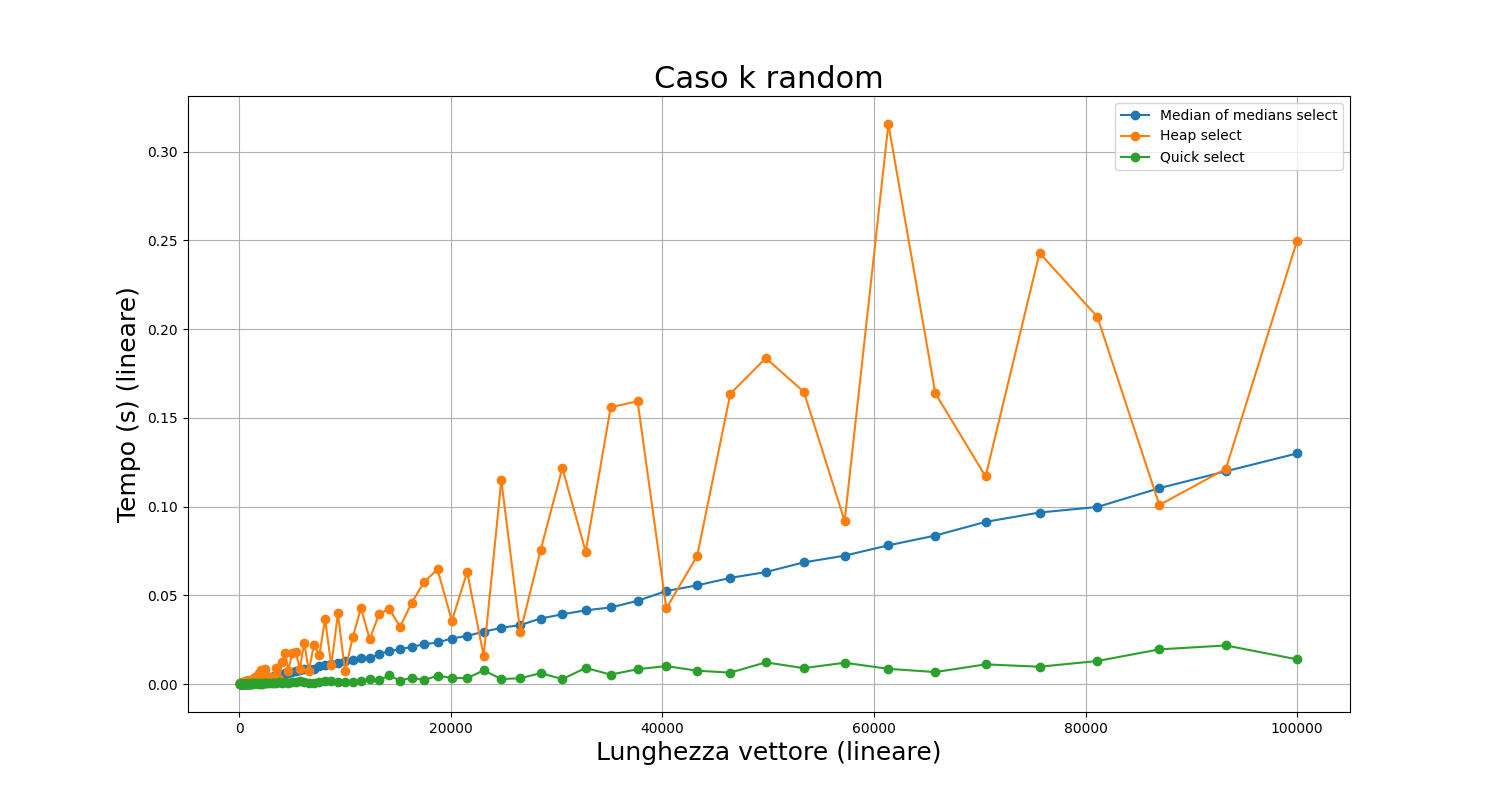
\includegraphics[width=.83\textwidth]{graphs/k_random_n.png}
            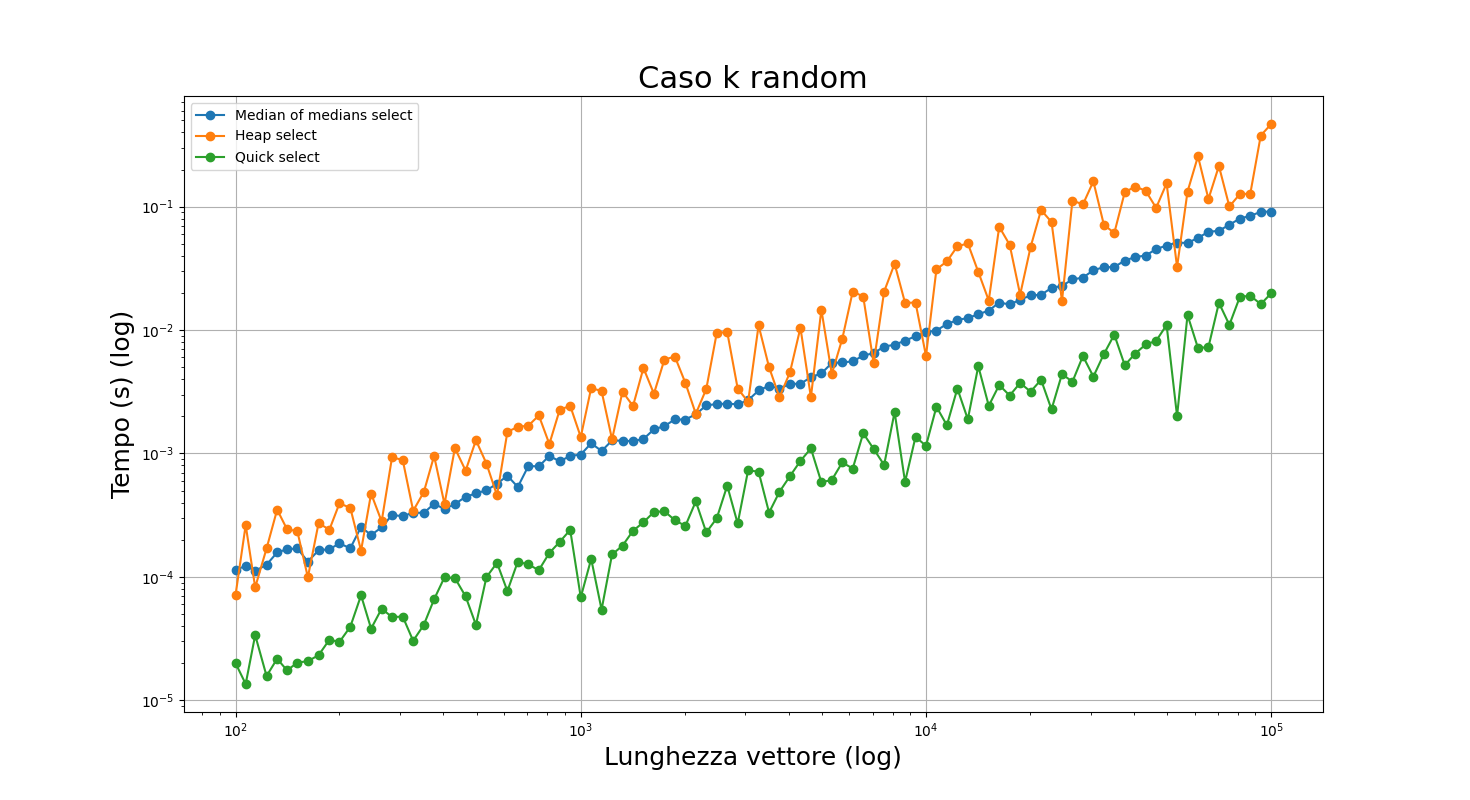
\includegraphics[width=.83\textwidth]{graphs/k_random_2xlog.png}
\end{figure}
Dai grafici soprastanti e da quelli precedente mostrati si rende ancora più evidente la quasi indipendenza di $MoM$ e $Quick\ Select$ dalla posizione di k. Al contrario invece si evidenzia la netta dipendenza della complessità di $Heap\ Select$ dovuta dalla posizione di k e in questo caso la sua imprevedibilità.\\
\newpage
\subsection{Caso n fissato e k variato}
\begin{figure}[h]
    \centering
    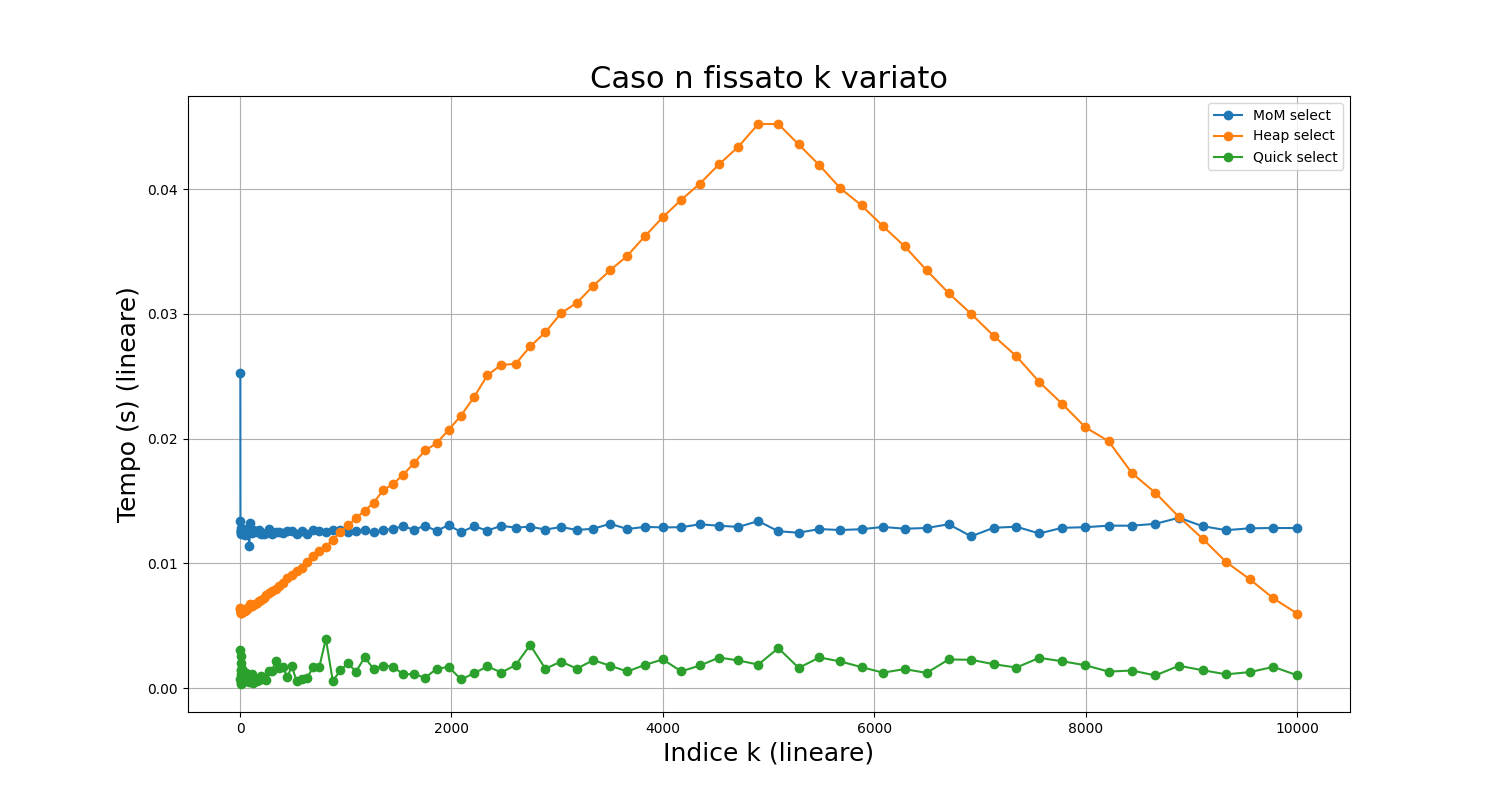
\includegraphics[width=.83\textwidth]{graphs/n_fixed_n.png}
    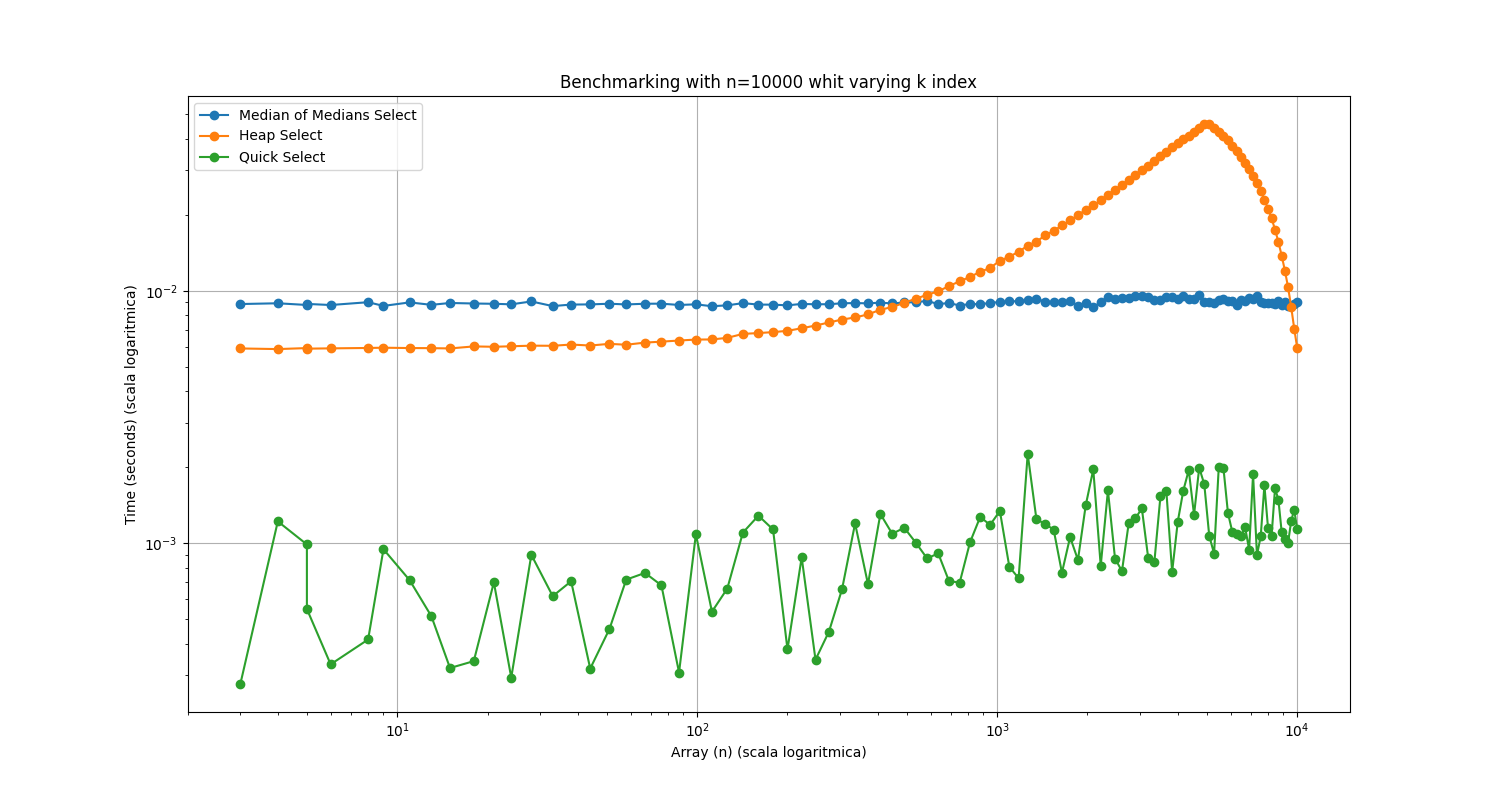
\includegraphics[width=.83\textwidth]{graphs/n_fixed_2xlog.png}
\end{figure}
Da questi particolari grafici con k varia seguendo una serie geometrica, che permette di distribuire i suoi valori in maniera esponenziale, mentre la lunghezza del vettore è fissa a n=10000. Si noti in maniera ancora più marcata della totale dipendenza dell'andamento di $Heap\ Select$ al valore k, difatto l'algoritmo mostra un comportamento monotono crescente per $k\in[0,\frac{n}{2}]$ raggiungendo un massimo a $k=\frac{n}{2}$. 
Successivamente l'algoritmo mostra un andamento monotono decrescente per $k\in[\frac{n}{2}+1,n-1]$, andandosi ad allineare con $MoM$ all avvicinarsi agli estremi del vettore. Riguardo ad $Quick\ Select$ e $MoM$ non traspare nulla di differente da quello che abbiamo già evidenziato nelle sezioni precedenti.\\
\newpage

\section{Confronto tra MoM}
\label{sec:confronto-mom}
\begin{figure}[h]
    \centering
    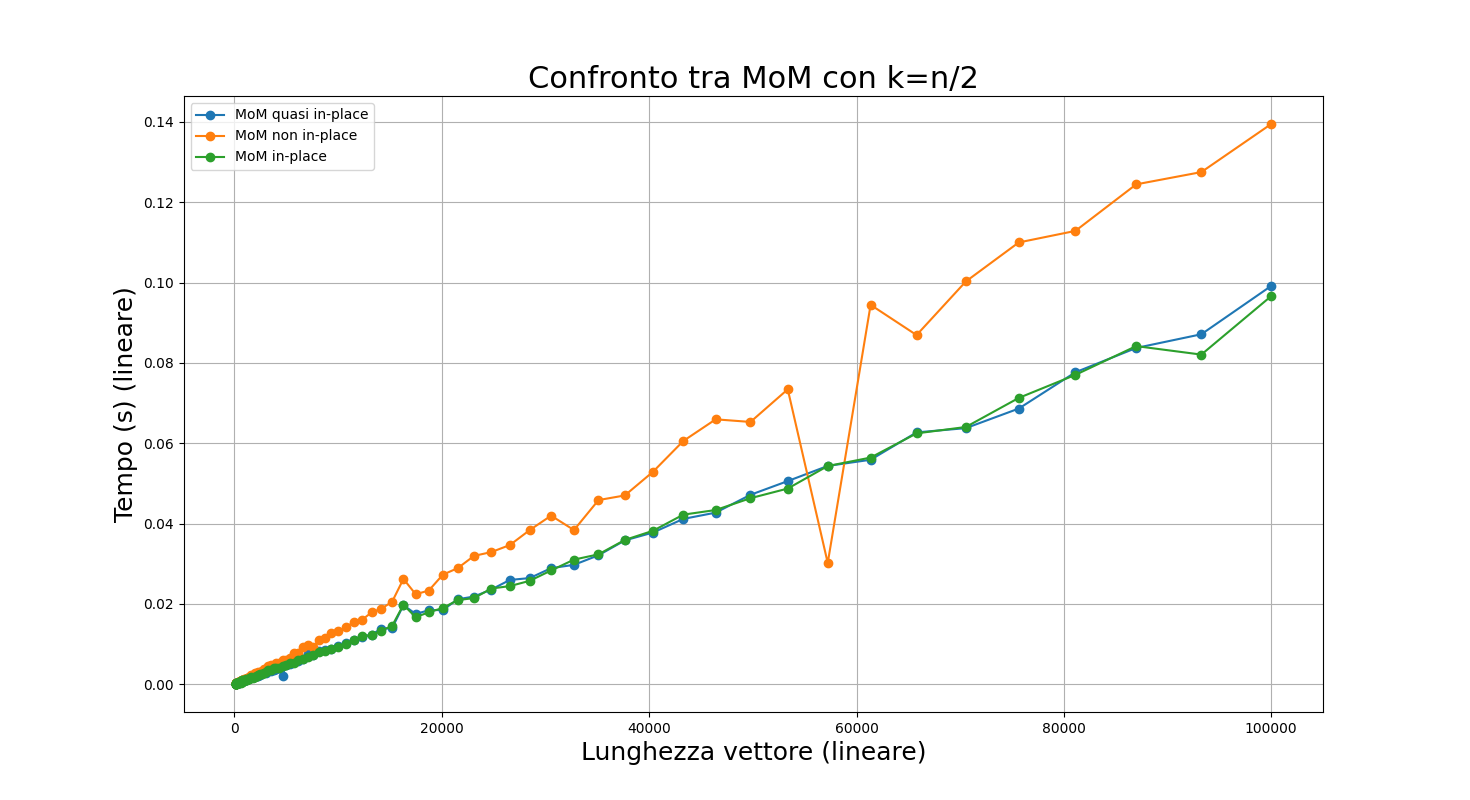
\includegraphics[width=.83\textwidth]{graphs/MoMs_n.png}
    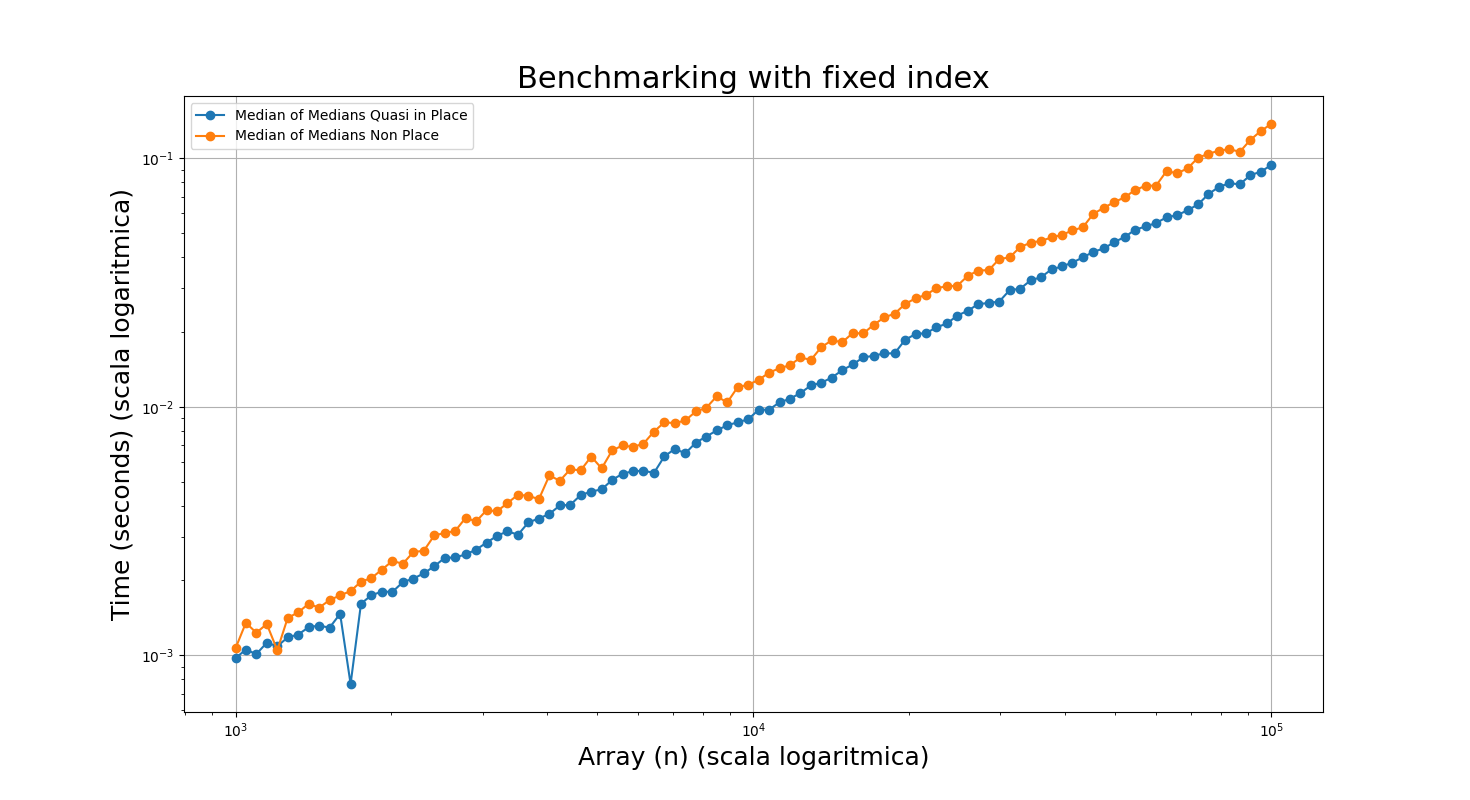
\includegraphics[width=.83\textwidth]{graphs/MoMs_2xlog.png}
\end{figure}
Come si può notare i due algoritmi hanno degli andamenti molto simili. La versione non in place a causa delle chiamate ricorsive e dell'utilizzo di due array supplementari si rivela essere meno prestante al crescere della lunghezza dell'array.
\end{document}